\begin{frame}
  \frametitle{Restbudget}
  \begin{columns}
    \column{0.7\linewidth}
      \begin{figure}
        \centering
		    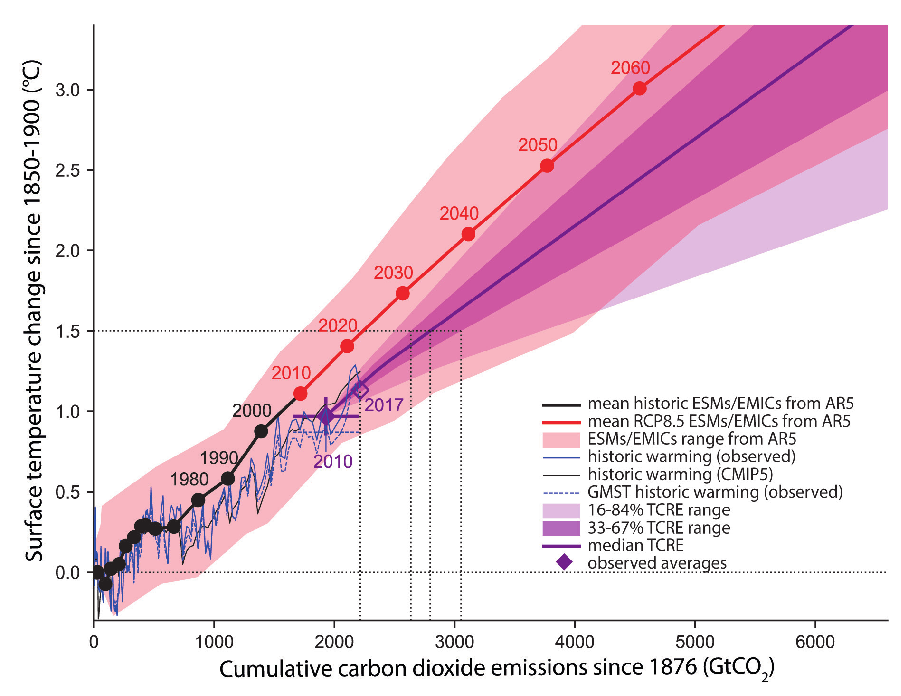
\includegraphics[width=\linewidth]{bilder/cumulative_co2.pdf}
		    \caption{Globale Oberflächentemperatur gegen kumulative CO$_2$-Emissionen.}
      \end{figure}
    \column{0.3\linewidth}
      \begin{itemize}
        \item Menge verbleibender Emissionen zur Begrenzung der Temperaturerhöhung
        \item Auf Basis von RCP8.5 Szenario des IPCC (business-as-usual)
        \item Auf Basis von Szenarien, die die globale Erderwärmung bis 2100 auf 1,5°C erreichen
      \end{itemize}
    \end{columns}
\end{frame}

\begin{frame}
	\frametitle{CO$_2$ Restbudget für Erwärmung um 1,5°C}
    \begin{itemize}
        \item Emission von maximal 420 GtCO$_2$ zur Einhaltung mit 66\%iger Warscheinlichkeit
        \item Emission von maximal 580 GtCO$_2$ zur Einhaltung mit 50\%iger Warscheinlichkeit
        \item Reduktion um 100 GtCO$_2$ bei Berücksichtigung von Erdsystem-Rückkopplungen wie Auftauen von Permafrostböden
        \item Globale Emissionen in 2019 49 GtCO$_2$eq % https://edgar.jrc.ec.europa.eu/overview.php?v=booklet2019
        \item Bei gleichgbleibender Rate sind die Restbudgets in 8,5 bzw. 11,8 Jahren aufgebraucht
    \end{itemize}

	\note{
		\begin{itemize}
			\item Restbudgets einerseits aus Erwärmung im Vergleich zu 1861-1880 auf Basis des RCP8.5 Szenarios
            \item Andererseits \"from a set of available pathways that were assessed to have a >50\% probability to exceed 1.5°C by mid-century, and return to 1.5°C or below in 2100 with greater than 66\% probability\"
            \item Weitere Studien, die teilweise nur CO$_2$ berücksichtigen
            \item Seit dem AR5 Report 2014 viele weitere Veröffentlichungen, die berücksichtigt werden
            \item Viele Unsicherheiten auf die berechneten Restbudgets wie Unterschiede in Szenarien zur Entwicklung von nicht-CO$_2$ Emissionen oder die Unsicherheit auf die historische Temperatur von 1850-1900
		\end{itemize}
	}
\end{frame}

\begin{frame}
  \frametitle{CO$_2$-Emissionen Deutschlands}
  \begin{columns}
    \column{0.7\linewidth}
      \begin{figure}
		    \centering
		    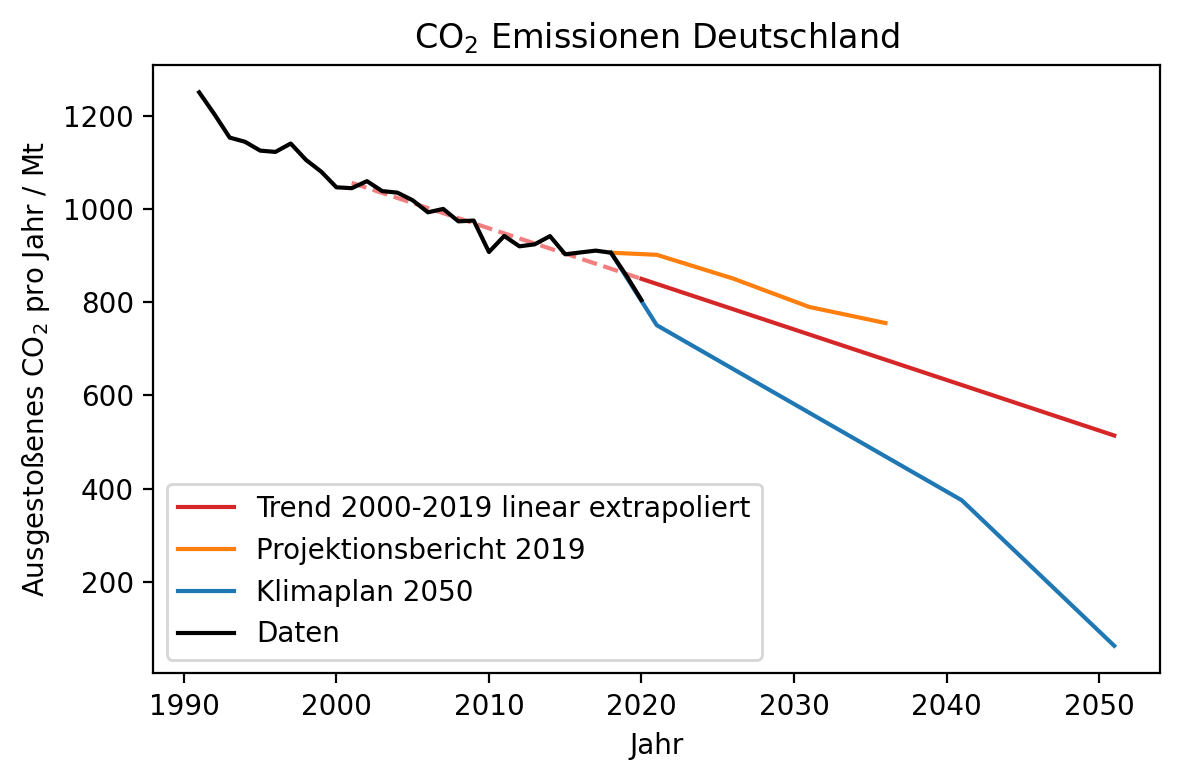
\includegraphics[width=\linewidth]{bilder/co2-emissions-de.png}
		    \caption{CO$_2$-Emissionen.}
      \end{figure}
    \column{0.3\linewidth}
      \begin{itemize}
        \item Bei linearer Fortsetzung: \enquote{0-Emissionen} erst in ca. 80 Jahren.
        \item Die deutschen Klimaschutzmaßnahmen sind nicht zielführend (Projektionsbericht).
        \item Klimaplan 2050 (Pariser Abkommen) zeigt ambitionierten Weg.
        \item[$\rightarrow$] Unklar, wie dieser Weg gegangen werden soll.
      \end{itemize}
    \end{columns}
\end{frame}

\begin{frame}
  \frametitle{Wie viele Emissionen stehen Deutschland noch zu?}
  \begin{columns}
    \column{0.7\linewidth}
      \begin{figure}
		    \centering
		    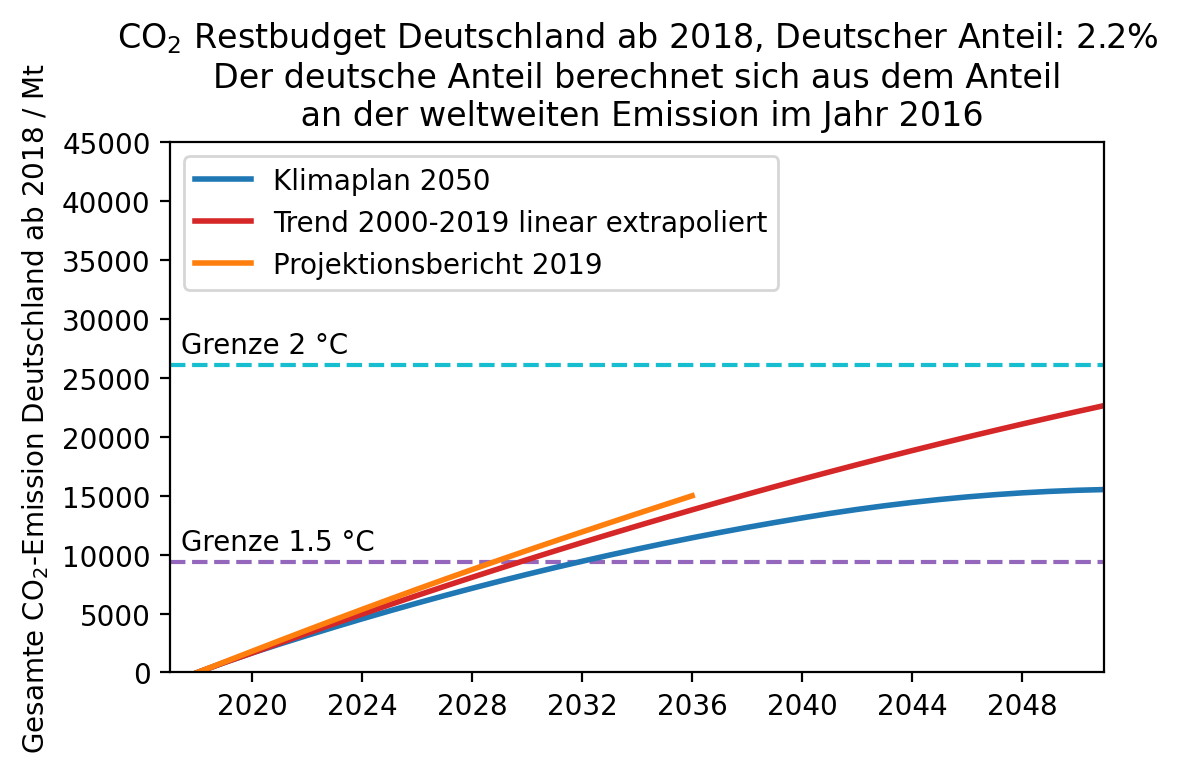
\includegraphics[width=\linewidth]{bilder/restbudget_de_new.png}
		    \caption{Globale Oberflächentemperatur gegen kumulative CO$_2$-Emissionen.}
      \end{figure}
    \column{0.3\linewidth}
      \begin{itemize}
        \item Die Bundesregierung geht davon aus, dass Deutschland aus den globalen CO$_2$-Budgets, die vom IPCC errechnet wurden ca. 2.2\% zustehen.
        \item Danach darf Deutschland pro Kopf doppelt so viel CO$_2$ ausstoßen, wie der durchschnittliche CO$_2$-Ausstoß pro Person auf der Welt ist.
      \end{itemize}
    \end{columns}

\end{frame}
